\chapter{Progress towards studies of quantum magnetism}
\label{ch:chap6}

A straightforward extension of the work presneted in this thesis would be to control interparticle spacing via an optical lattice. For these and additional experiments using quantum degenerate fermionic strontium we purchased and installed an optical lattice system. Our lattice is implemented using a Coherent Verdi V-18 which is shapped and propagated to our science chamber in free space. \hl{Fig} shows the optical path for each arm of our cubic lattice. 

Unfortunately, complications due to heating when loading the lattice has limited our success in this optical trap. I want to go over what we have been able to do so far with the lattice.

How did we characterize?
	Kaptiza-dirac extension
	
What convinced us we were having problems?

What are some ideas we could do in the lattice?
	Zeno
	faster cooling via stimulated raman potentailly? (can I model this somehow?)
	repulzively bound molecules?
	use interaction control in lattice with the zeno thing
	
	

\section{532 nm optical lattice: installation and characterization}
\label{sec:lattice}

Optical lattices are formed by a standing wave of light which creates a defect free periodic potential. These traps are extremely versatile and have enabled the observation of the superfluid - Mott insulator transition \cite{Greiner2002}, artificial gauge fields for neutral atoms \cite{Lin2011}, quantum microscopy with single-site resolution \cite{Bakr2009}, and investigations of quantum magnetism \cite{Hart2015,Greif2015}. They are among the most well-established techniques for controlling a quantum state and have proven to be great tools for exploring the connection between few- and many-body systems \cite{Bloch2008}.

\subsection{Background}
\label{ssec:lattice_background}

This section should cover band structure and refer to the types of wavefunctions that are possible. Perhaps through some stuff in here from the quantum magnetism proposal from the NSF 

Until recently, experiments on the Neutral apparatus were confined to work with bulk gases in an optical dipole trap. While optical dipole traps are useful for efficient evaporation and thermalization of an ultracold gas, experiments with Feshbach molecules in ODTs suffer from a high rate of inelastic collisions. \cite{Kohler2006}. The association of these molecules in an optical lattice has been shown to slow these processes since atoms must tunnel from site to site and can be pinned in sufficiently deep potentials \cite{Thalhammer2006,Syassen2007}. In order to gain a quantitative understanding of these processes we will briefly outline the relevant lattice physics for ultracold bosons in an optical lattice.

An optical lattice is created by counterpropagating two laser beams to form a standing wave pattern, which for two plane waves in one dimension results in a periodic potential given by 
	\begin{equation} \label{eq:1dlattice}
		 V(x) = V_{lat} \; \sin^2(k_L x)
	\end{equation}
where $V_{lat}$ is the lattice depth determined by the polarizability of the atom for a given trapping wavelength $\lambda$ and laser intensity $I$, and $k_L$ is the lattice wavevector . This potential can be readily extended to three dimensions using two additional pairs of counterpropagating laser beams along the $y$ and $z$ directions which results in a 3D cubic lattice. Depth of the trapping potential, $V_{lat}$, is controlled by varying the intensity of the lattice beams. Clever arrangements of laser beam propagation, in addition to phase and polarization control of the trapping fields, can extend these standing wave potentials to a number of non-trivial geometries such as triangular, checkerboard, and dimerized lattices \cite{Greiner2003}.

Periodic potentials are powerful because they break the translational invariance of space which results in the formation of band structure and the opening of bandgaps or disallowed particle energies \cite{Ashcroft1976}. Because of the broken invariance, $p$ is no longer a good quantum number and instead must be replaced by two new quantum numbers: the band index, $n$, and the quasimomentum, $q$. In one dimension, quasimomentum is specified by $q = p - nG$, where $G=2\pi/a$ is a reciprocal lattice vector, and $a$ is the real space lattice constant. Fig.\;\ref{fig:bandStructure} shows how the band structure varies as the lattice depth is increased. Optical lattices have a lattice spacing $a = \lambda /2$ which determines the reciprocal lattice vector $G = 4\pi / \lambda = 2 \hbar k_L$ and the natural energy scale $E_r = \frac{\hbar^2 k_L^2}{2m}$ where $m$ is the atomic mass and $k_L$ is the lattice wavevector, $k_L = 2\pi / \lambda$. From the band structure, we see that the bandwidth of each band, given by $\Delta E = E_{q=\hbar k_L} - E_{q=0}$, decreases as the lattice depth is increased. In the limit that $V_{lat}\!\rightarrow\!\infty$ the band structure reduces to a ladder of harmonic oscillator levels spaced by $\hbar \omega_{ho} = \sqrt{4 V_{lat} E_r}$. Although, for moderately deep lattices, $V_{lat} \gtrsim 5\,$E$_r$, this approximation is valid near the center of the Brillioun zone, $q = 0$, and provides a simple form to estimate the energy gaps between bands \cite{Jaksch1998,Jaksch2005}.


\begin{figure} \label{fig:bandStructure}
	\centerline{
	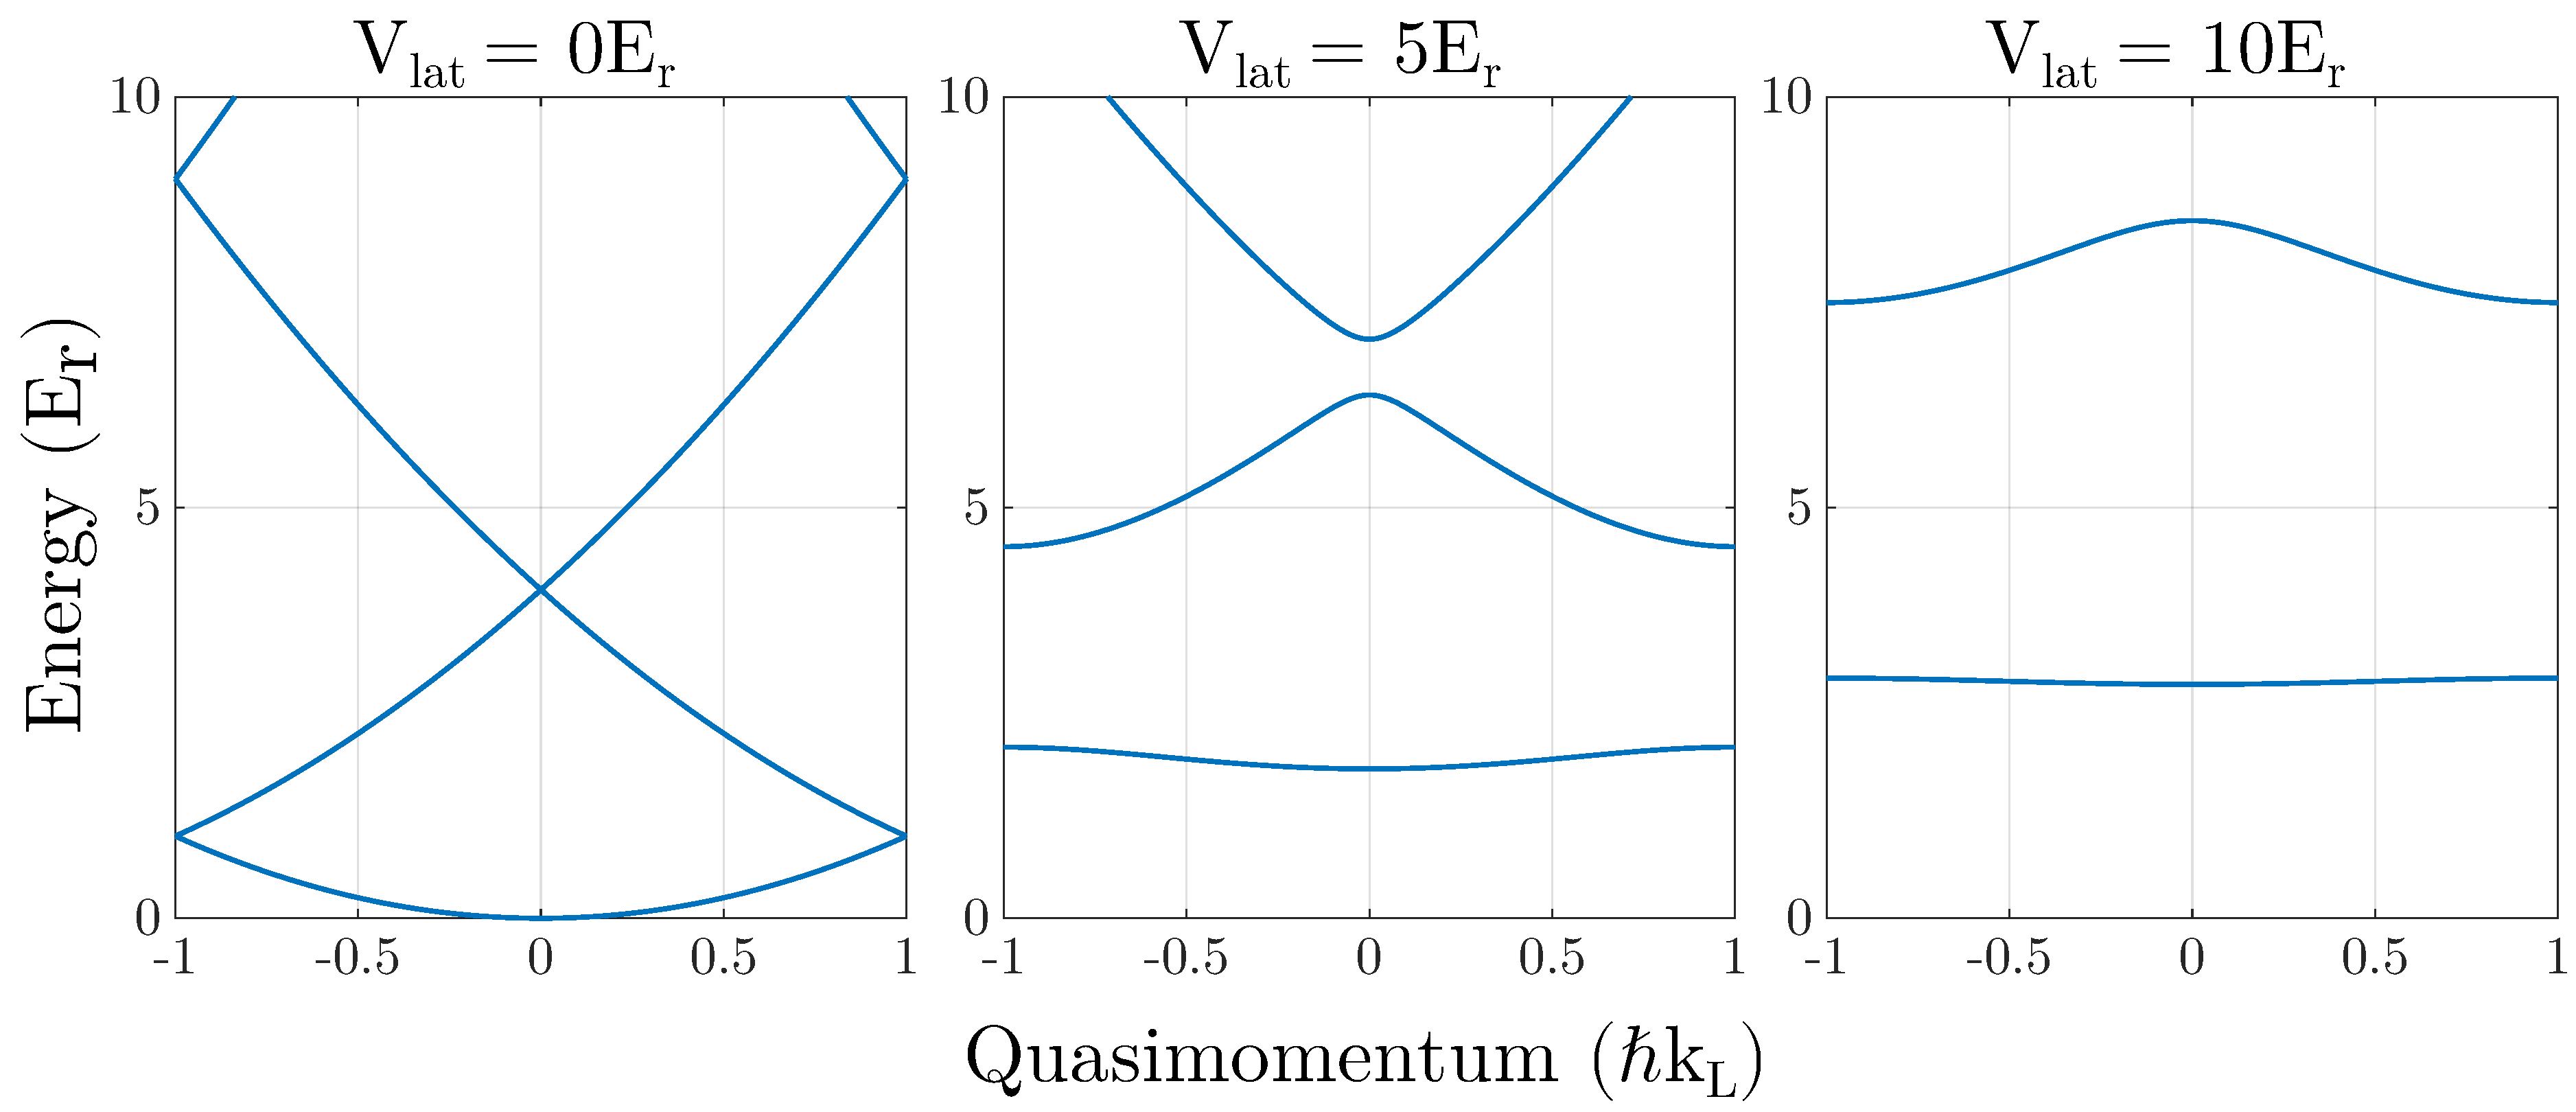
\includegraphics[width=\textwidth]{Fig2_bandStructure.pdf}}
	\caption{1D band structure as a function of lattice depth}{One dimensional band structure for an optical lattice as the lattice depth is increased. The band energies are found by solving the Schr\"{o}dinger equation using the Bloch functions of Eq.\;\ref{eq:blochFunc}.}
\end{figure}
	
	
Solutions to the Schr\"{o}dinger equation in a periodic potential are given by the Bloch functions \cite{Ashcroft1976}
	\begin{equation} \label{eq:blochFunc}
		 \phi_q^{(n)}(x) = e^{iqx/ \hbar} \; u_q^{(n)}(x)
	\end{equation}
These eigenstate wavefunctions are specified for a given quasimomentum $q$, and band index $n$. Their corresponding energy eigenvalues define the band structure of the lattice shown in Fig.\;\ref{fig:bandStructure}. From Eq.\;\ref{eq:blochFunc} we see that the Bloch functions are the product of plane waves modulated by a function $u_q^{(n)}(x)$, which shares the periodicity of the underlying lattice potential \cite{Ashcroft1976}. For an optical lattice this modulating function can be expanded in a basis of plane waves through a Fourier decomposition of the lattice potential in Eq.\;\ref{eq:1dlattice}, which gives \cite{Greiner2003},
	\begin{equation} \label{eq:blochMod}
		 u_q^{(n)}(x) = \sum_l c_l^{(n,q)} \; e^{i2lk_Lx}
	\end{equation}
Here $c_l^{(n,q)}$ are the coefficients for each plane wave in the basis expansion that are found by diagonalizing the lattice Hamiltonian \cite{Greiner2003}.

Often, we are interested in the dynamics of particles on a particular lattice site, but since Bloch functions are delocalized pver the entire lattice, it is useful to instead use the Wannier functions. These functions provide an orthogonal and normalized set of wavefunctions that are maximally localized to a specific lattice site. The Wannier function for a localized particle in the n$^{th}$ band of a lattice site located at position x$_i$ is given by \cite{Jaksch2005}
	\begin{equation} \label{eq:wannier}
		 w_{n}(x - x_i) = \mathcal{N}^{-1/2} \sum_q e^{iqx_i/ \hbar} \; \phi_q^{(n)}(x)
	\end{equation}
where $\mathcal{N}$ is a normalization constant and $\phi_q^{(n)}(x)$ are the Bloch functions of Eq.\;\ref{eq:blochFunc}. This localized description of particles allows us to calculate important physical quantities which govern dynamical properties of the lattice such as the tunneling rate, $J/ \hbar$, and on-site interaction energy, $U$.  As $V_{lat}\!\rightarrow\!\infty$, the Wannier functions approach the eigenfunctions of the harmonic oscillator, which allows us to estimate the spatial extent of an atomic wavefunction by $a_{ho} = \sqrt{\frac{\hbar}{m \omega_{ho}}}$ \cite{Jaksch2005}. 

When bosons are confined to the lowest energy band of a lattice, a particularly simple model known as the Bose-Hubbard Hamiltonian is used to describe the lattice system \cite{Jaksch1998}. 
	\begin{equation} \label{eq:boseHubbard}
		 H_{BH} = -J \sum_{\left< i,j \right>} \left(\hat{b}^{\dagger}_i \hat{b}_j + \hat{b}^{\dagger}_j \hat{b}_i \right)
		 		  + \frac{U}{2} \sum_i \hat{n}_i(\hat{n}_i - 1)
	\end{equation}
Where $\left< i,j \right>$ denotes a sum over nearest-neighbors. This model is the simplest example of a non-trivial interacting many-body system for dynamics in a lattice. The first term describes hopping of bosons from site to site at a rate $J/ \hbar$. The second term describes an interaction energy which is related to the s-wave contact interaction term, $g = 4 \pi \hbar^2 a_s/m$, where $a_s$, is the s-wave scattering length of the particles. $J$ and $U$ can be calculated directly using the Wannier functions of Eq.\;\ref{eq:wannier} and are given by \cite{Jaksch2005}
	\begin{equation} \label{eq:JandU}
	\begin{aligned}
		 J_{ij} &= - \int d^3x \; w_0(x-x_i) \left( \frac{p^2}{2m}+V(x) \right) w_0(x-x_j)\\
		 U &= \frac{4 \pi \hbar^2 a_s}{m} \int d^3x \; \left| w_0(x-x_i)\right|^4
	\end{aligned}
	\end{equation}
Using Eq.\;\ref{eq:JandU} we have calculated the expected tunneling rates and interaction energies for atomic strontium and plot the results in Fig.\;\ref{fig:fig_JandU} for homonuclear samples of strontium as a function of lattice depth. This single band calculation is valid under the assumption that the interaction energy of a site is smaller than the bandgap between the $n= 0$ and $1$ bands, namely $U N \lesssim \hbar \omega_{ho}$ where $N$ is the mean number of particles per site and $\hbar \omega_{ho}$ is the approximate energy spacing between bands \cite{Rey2004}. 


\begin{figure} \label{fig:fig_JandU}
	\centerline{
	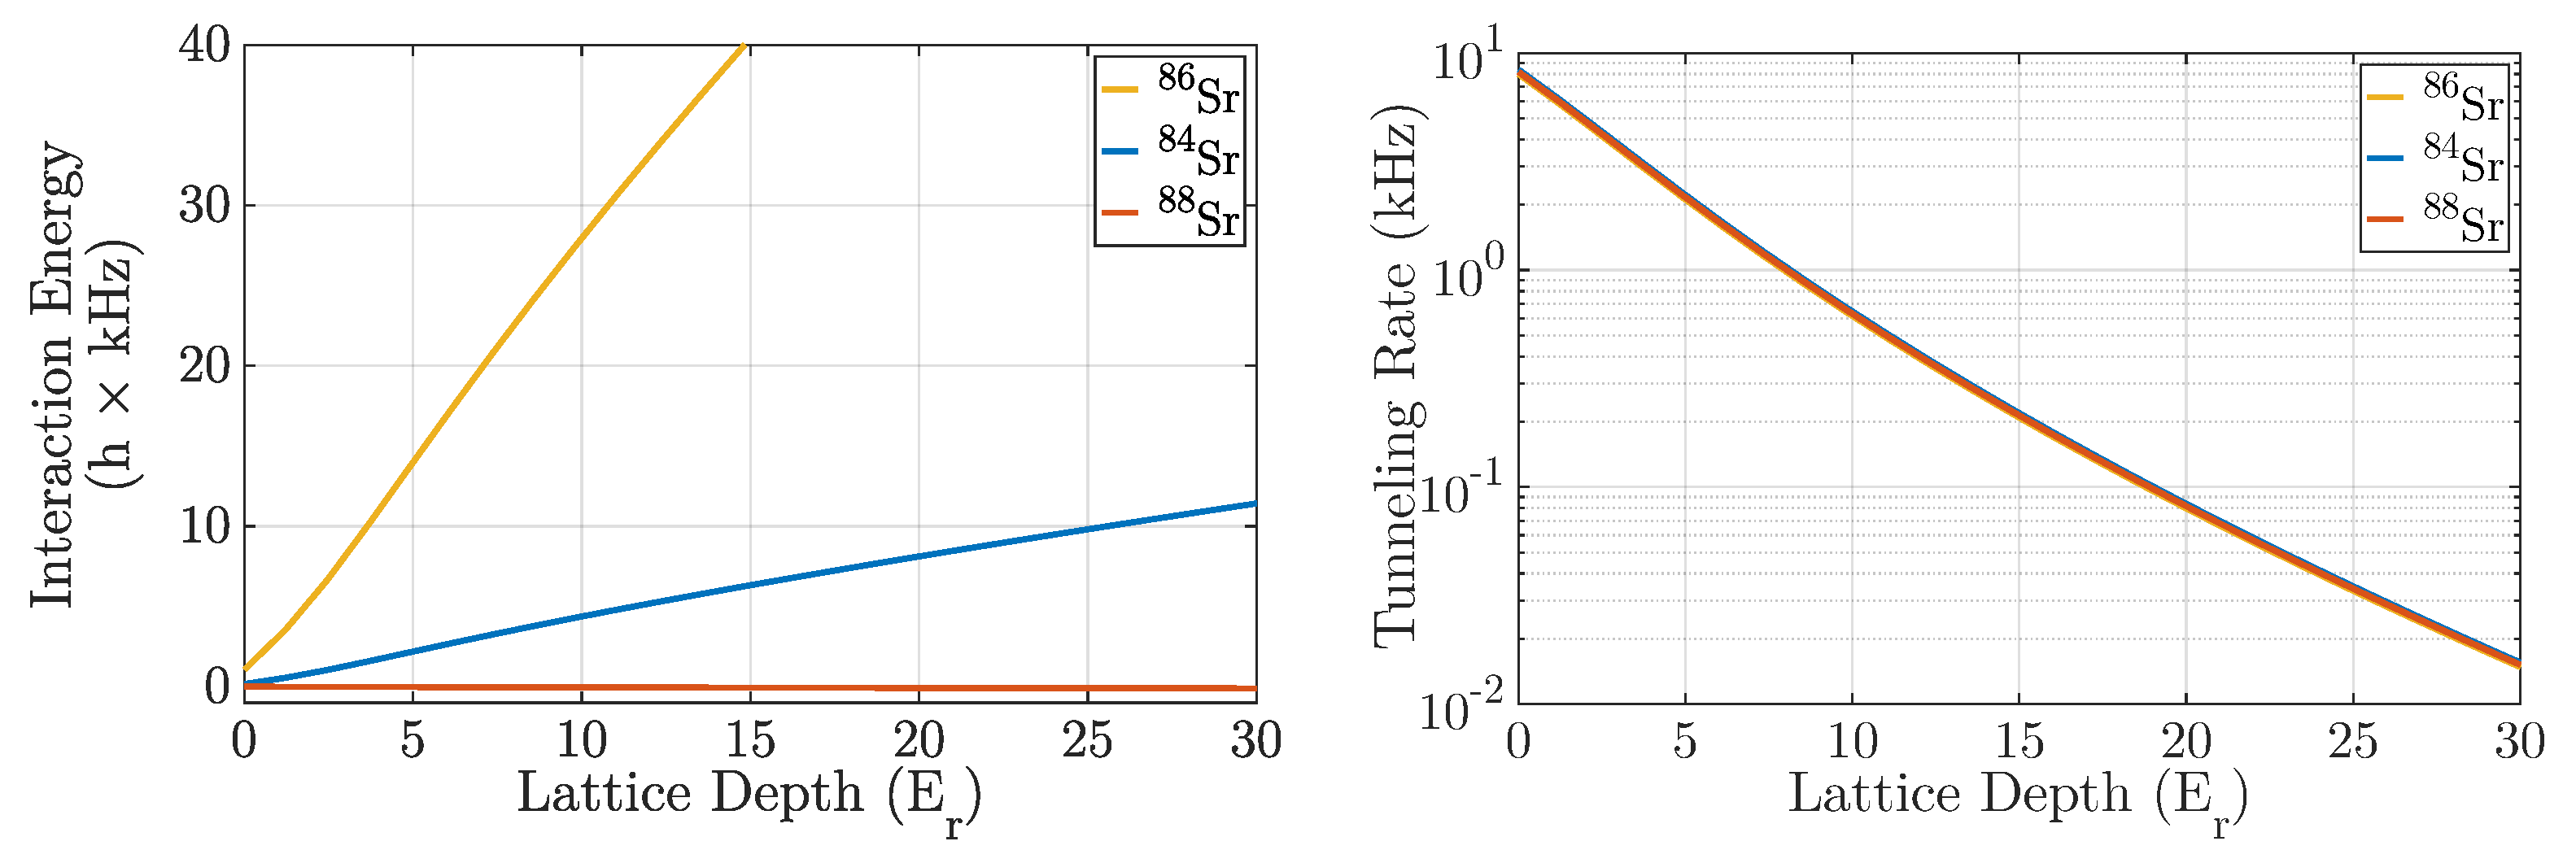
\includegraphics[width=\textwidth]{Fig3_JandU.pdf}}
	\caption{Calculated interaction energies and tunneling rates for each isotope of strontium}{The interaction energy shows a large variation because of its dependence on the s-wave scattering length. However, the tunneling rate is approximately the same for all isotopes since the change in mass is negligible between isotopes.}
\end{figure}
	
	
Alternatively, Eq.\;\ref{eq:JandU} can be simplified through considering appropriate limits to the Bose-Hubbard model. In the limit that $U\!\rightarrow\!0$, the Bose-Hubbard model becomes exactly solvable and the energy of the $n=0$ band is given by $E_q^{(0)}=-2J \cos(q a)$ \cite{Jaksch2005}. Thus, the tunneling rate, $J$, can be related to the bandwidth of the lowest band as expressed in Eq.\;\ref{eq:JandU_simple}. Under a separate limit, $V_{lat}\,\rightarrow\,\infty$, then the tunneling rate goes to zero and the localized wavefunctions can be approximated by a Gaussian wavefunction which yields the form for the on-site interaction $U$ given in Eq.\;\ref{eq:JandU_simple} \cite{Rey2004}.
	\begin{equation} \label{eq:JandU_simple}
	\begin{aligned}
		 J &= \frac{E_{q=\hbar k_L} - E_{q=0}}{4}\\
		 U &= \frac{\hbar a_s}{\sqrt{2 \pi}}\frac{\bar{\omega}_{ho}}{\bar{a}_{ho}}
	\end{aligned}
	\end{equation}
Here $\bar{a}_{ho}$ and $\bar{\omega}_{ho}$ are the geometric means of the one-dimensional harmonic oscillator length and frequency given previously.

Competition between $J$ and $U$ results in a phase transition known as the superfluid - Mott insulator transition \cite{Fisher1989,Greiner2002}. When $J/U \gg 1$ atoms are free to delocalize over the lattice and the many-body ground state is a superfluid. In the opposite limit that $J/U \ll 1$, particle fluctuations between sites are no longer energetically accessible and the system transitions into an interaction induced insulating state known as a Mott insulator. This state is characterized by fixed particle number per site and in a 3D cubic lattice near unit filling, this phase transition occurs at $J/U \approx 35$ which, for $^{84}$Sr, corresponds to a lattice depth of $V_{lat} \approx 13E_r$ \cite{Fisher1989}.

The tunability of an optical lattice potential is useful for studying feshbach molecules. By controlling the lattice depth and/or atomic density, we can efficiently create molecules when there are two or more atoms per site. Using the volume of a unit cell we can estimate the densities needed to reach average on-site occupancy of 2, which is ideal for forming isolated molecules. For a lattice wavelength of 532\,nm in a simple cubic configuration, the volume for each lattice site is 1.9 $\times 10^{-14}\,$cm$^3$, so we must achieve densities on the order of $4 \times 10^{14}\,$cm$^{-3}$ to expect significant conversion. A more detailed approach to estimate our conversion efficiency would entail: 1) calculating the variation in chemical potential across the trap due to the inhomogeneous confinement of the trapping potential, 2) finding the average particle number per site as a function of $J/U$ to estimate the distribution of $\mu / U$ on the superfluid - Mott insulating phase diagram \cite{Fisher1989}, and 3) integrating the density distribution from the center of the trap to a limiting value of $\mu / U$, where the local density is too dilute for efficient molecule conversion. Though such a calculation is beyond the scope of this proposal, it is worth noting that the shell structure found near the Mott insulating regime inhibits complete molecular conversion of the atomic gas. Therefore, molecules are accompanied by a large number of unconverted remnant atoms. Previous investigators have shown that it is beneficial to clear non-molecule atoms out of the lattice through a sequence of light and/or microwave pulses. Such a cleaning sequence will need to be investigated in our system since tunneling from single atoms can lead to a reduction of the molecular lifetime \cite{Kohler2006,Thalhammer2006}.

\subsection{Setup}
\label{ssec:lattice_setup}

This section should cover all the specifics regarding the lattice

 Our optical lattice operates at $\lambda=532\,$nm and is derived from a Coherent Verdi V-18 single mode laser which is sent through separate AOMs for intensity control of each arm before propagating in free space to the atoms. The horizontal arms of the lattice ($x$ and $y$) have $1/e^2$ waists of $200\,\mu$m x $200\,\mu$m and their polarization is linear and aligned along the $z$ direction, parallel to gravity. The vertically propagating beam has a $1/e^2$ waist size of $300\,\mu$m x $300\,\mu$m and polarization aligned orthogonal to the polarization of the horizontal beams. With this configuration we have measured a maximum depth of $9$E$_r$ in an isotropic lattice. As this is our first implementation of an optical lattice, we have spent a significant amount of time characterizing our system as detailed below.


\subsection{Measurement and results}
\label{ssec:lattice_tests}

What are all the types of experiments we did in the lattice?

Cover sideband cooling and Bloch oscillations
Results, look into why its not necessarily so easy from end of red MOT, thoughts on how it could become useful

\subsubsection{Kaptiza-Dirac Scattering}
\label{sssec:sideband_cooling}

Brief intro to theory and some plots showing fits.


Fig.\;\ref{fig:KDoscillations} shows a typical Kapitza-Dirac oscillation pattern which we use to maximize beam overlap near the atoms and calibrate our achievable lattice depths. Kapitza-Dirac is useful as an alignment tool since measurement of the population oscillation frequency can be highly accurate and directly relates to the bandgap energy in the lattice, shown in Fig.\;\ref{fig:bandStructure}. 


\begin{figure} \label{fig:KDoscillations}
	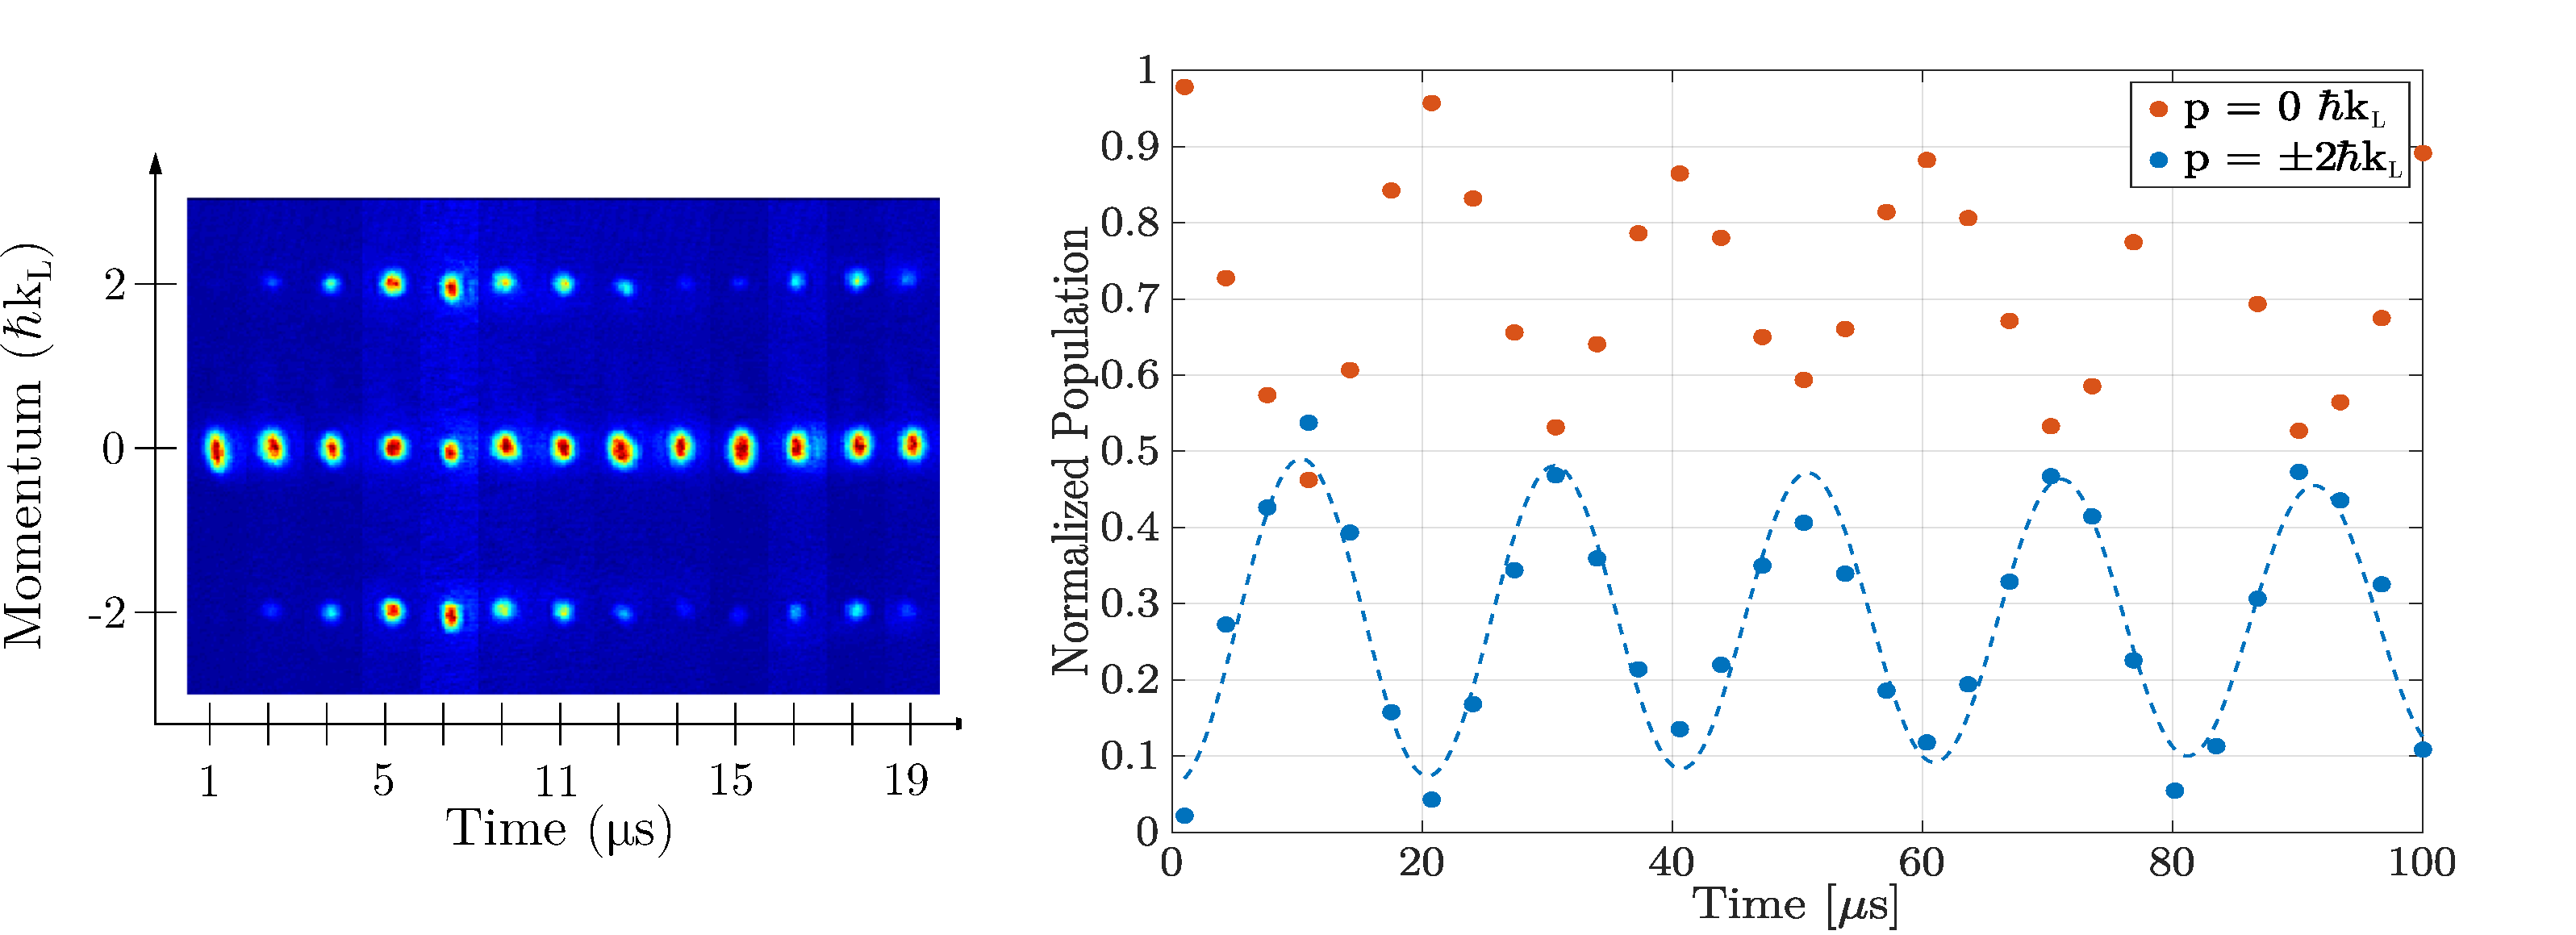
\includegraphics[width=\textwidth]{Fig7_kdOsc.pdf}
	\caption{Evolution of plane wave population using Kapitza-Dirac}{Left: Time of flight slices for several realizations of Kapitza-Dirac with varying hold time in the lattice. Right: Normalized population from fits of time-of-flight images. Oscillations are fit with a decaying sinusoidal and the best-fit frequency is used to determine the lattice depth.}
\end{figure}
	
	
Kapitza-Dirac diffraction can be viewed as a diabatic projection from an initial eigenstate to a new set of eigenstates which results in an oscillation of the wavefunctions probability amplitudes over the new eigenstates of the system \cite{Denschlag2002}. As was discusses in Sec.\;\ref{sec:lattice}, the free space eigenstates are not the eigenstates of the lattice Hamiltonian. Thus a pure $p=0$ plane wave, $\ket{\phi_{p=0}}$, suddenly loaded into an optical lattice can be written as a superposition of the Bloch states given by Eq.\;\ref{eq:blochFunc}, here denoted by \ket{n,q}.
	\begin{equation} \label{eq:p0inBloch}
		\ket{\Psi(t=0)} = \sum_{n=0}^{\infty} \ket{n,q} \innerProd{n,q}{\phi_{p=0}}
	\end{equation}
The time evolution of this state is then given by
	\begin{equation} \label{eq:KDtime}
		\ket{\Psi(t)} = \sum_{n=0}^{\infty} \ket{n,q} \innerProd{n,q}{\phi_{p=0}} exp \left( \frac{-i E_n(q) t}{\hbar} \right)
	\end{equation}
where $E_n(q)$ is the energy of the Bloch state at a specified $q$ and $n$ shown in Fig.\;\ref{fig:bandStructure}. The exponential factor of Eq.\;\ref{eq:KDtime} introduces oscillations among Bloch states and after a second diabatic projection back to the plane wave basis, we can relate evolution of plane wave population to the bandgap energy. From this analysis we find that for relatively weak lattices, $V_{lat} \lesssim 10 E_r$, the plane wave population will vary as $\omega_{osc} = (E_2 - E_0) / \hbar$. Where $E_i$ is the band energy of the i$^{th}$ band with $q=0$ as is the case when performing Kapitza-Dirac with a Bose-Einstein condensate.


\begin{figure} \label{fig:heatingRates}
\centerline{
	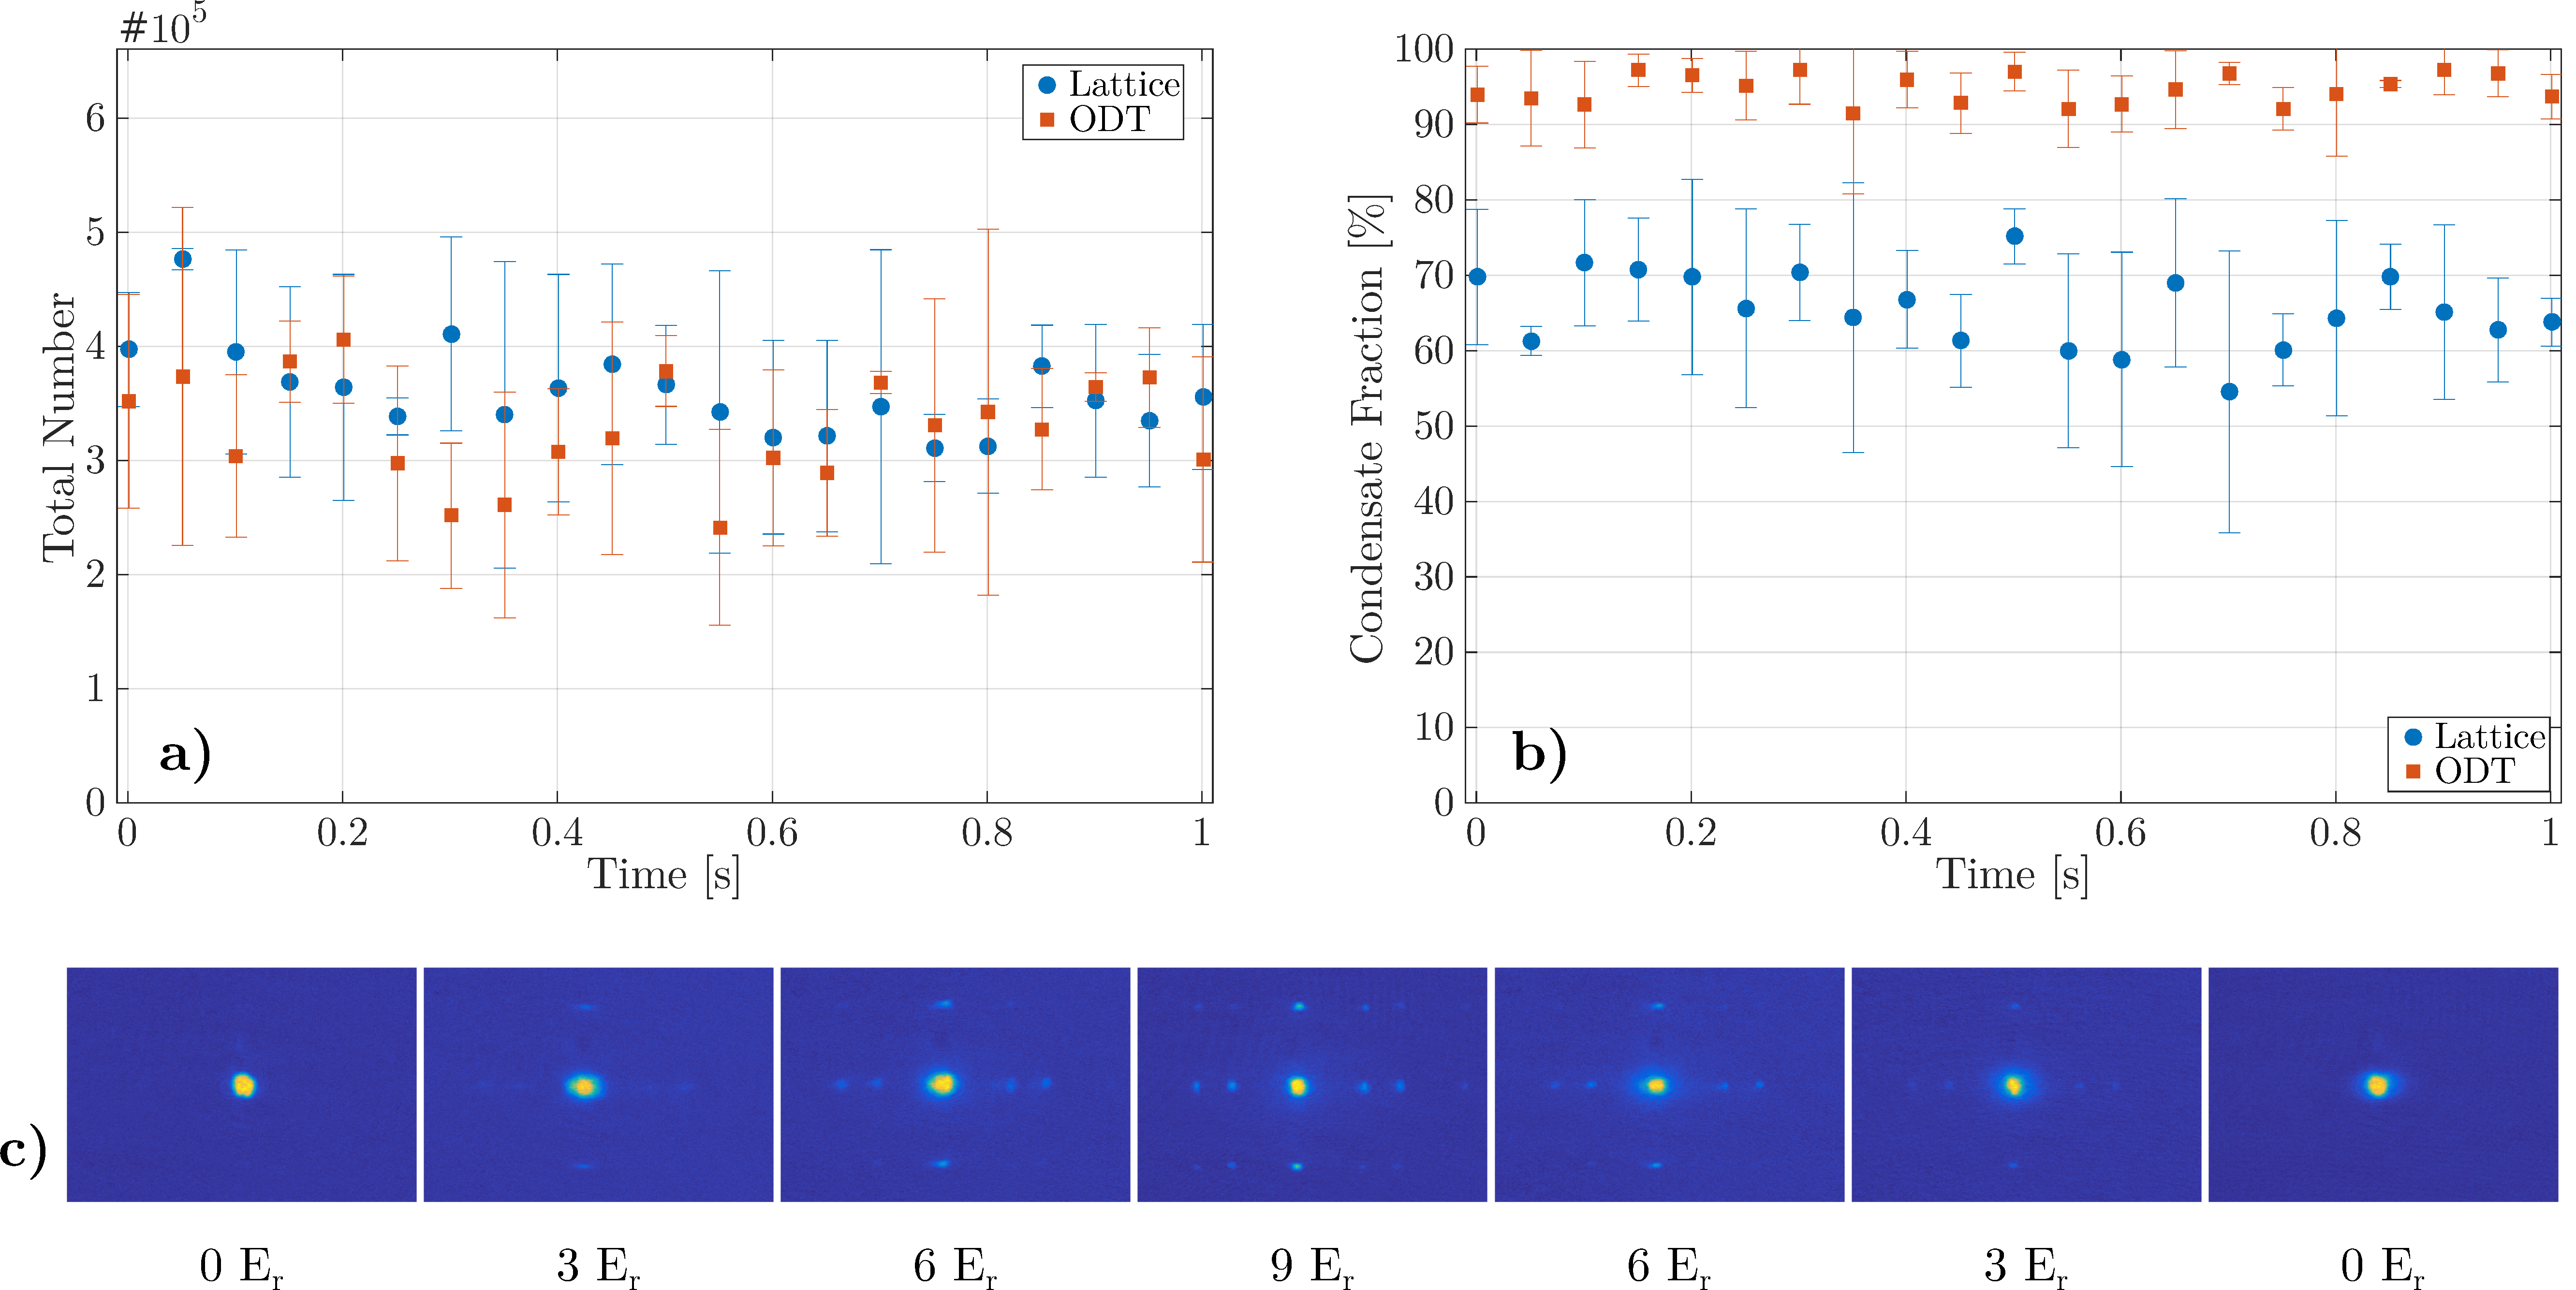
\includegraphics[width=\textwidth]{Fig8_heatRates.pdf}}
	\caption{Evolution of condensate fraction over time after adiabatically ramping on the lattice to 9\,E$_r$. a,b) Comparison of total number and condensate fraction for a sample held in the optical dipole trap (red squares) or in a deep lattice (blue circles). c) Time of flight images after ramping on the lattice and diabatically projecting back to plane wave states. }
\end{figure} 
	


\subsubsection{Heating of a quantum degenerate gas}
\label{sssec:sideband_cooling}

Creation of a Mott insulator and the results showing unacceptable heating rates

While Kapitza-Dirac diffraction is useful as a characterization tool, we typically wish to maintain equilibrium when loading condensates into the lattice. Thus slowly ramping up the lattice laser intensity will adiabatically transform a plane wave ground state into the ground Bloch state of the lattice \cite{Sakurai2010}. Strictly speaking, in order to adiabatically connect the free space eigenstates and the lattice eigensates, the lattice must be turned on infinitely slowly due to the infinitesimal bandgaps which open near the band edges. Although near the band center, $q=0$, the adiabaticity requirement relaxes to $dV_{lat}/dt \ll 16E_r^2/ \hbar$, \cite{Denschlag2002} which for strontium in a 532\,nm lattice is $\approx 5\,\mu$s$/E_r$. However, in practice we find that our condensate fraction is reduced during fast ramps into the lattice. Instead, we exponentially ramp on the lattice over $100\,$ms which reduces heating caused by the ramp. As shown in Fig.\;\ref{fig:heatingRates}, we observe a large condensate fraction after similarly ramping the lattice back down. Additionally, by holding in a deep lattice after an adiabatic ramp, we can measure the effects of off-resonant scatter of lattice photons as a reduction of atom population over time. For our red detuned optical lattice we expect the off-resonant scattering rate to be well approximated by a simple two level approach. In this model, the effective scattering rate is given by \cite{Jaksch2005}
	\begin{equation} \label{eq:offResScatter}
		\Gamma_{eff} \approx \frac{\Gamma V_{lat}}{\hbar \delta_{lat}}
	\end{equation}
where $\Gamma$ is linewidth of the dipole transition between the two states, $V_{lat}$ is the lattice depth, and $\delta_{lat}$ is the detuning of the optical lattice from the two level transition frequency. In strontium, the $^1S_0\!\rightarrow\!^1P_1$ transition strongly dominates the polarizability of the ground state and therefore can be used to estimate the effective off-resonant scattering rate. For this transition $\Gamma = 2 \pi \times 30.5\,$MHz and a 532\,nm lattice is detuned by $\delta_{lat} \approx 2 \pi \times 87\,$THz. With a lattice depth of $V_{lat}=10\,$E$_r$ we expect a scattering rate of $\Gamma_{eff} \approx 2\e{-1}\,$s$^{-1}$, which is negligible for the timescales of our proposed experiments. From Fig.\;\ref{fig:heatingRates}, we see that there is not an appreciable loss of atoms over a one second timescale, supporting our estimate that off-resonant scattering is unimportant on these timescales.


\begin{figure} \label{fig:oneColorSB}
	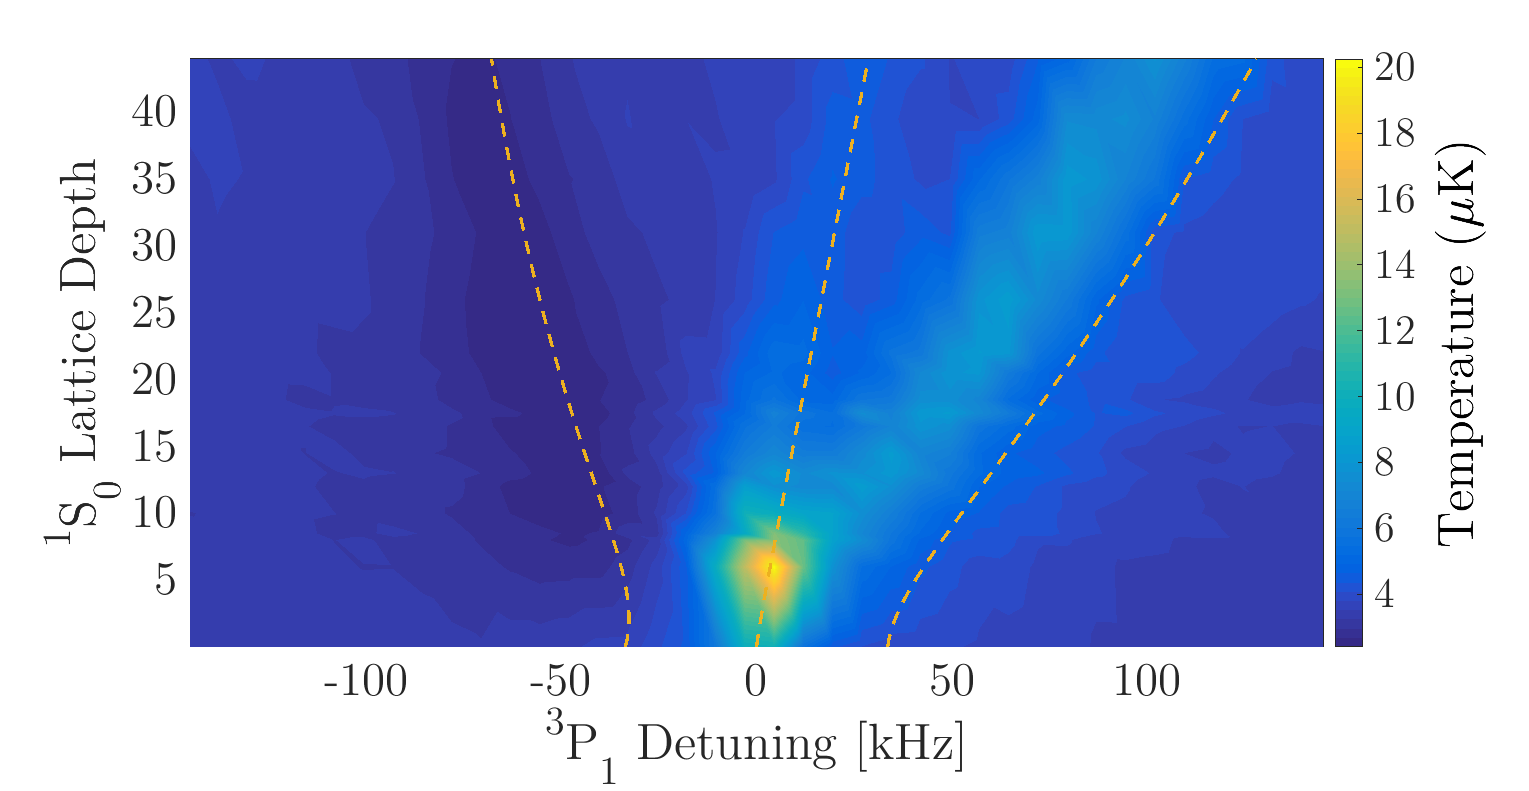
\includegraphics[width=\textwidth]{fig9_sidebands.png}
	\caption{Observation of driven sideband transitions}{Driven sidebands in a 1D lattice as a function of lattice depth using an ultracold gas with an initial temperature of $\approx 200\,$nK. Dashed lines are the expected band positions using a 1D model of the lattice as shown in Fig.\;\ref{fig:bandStructure}.}
\end{figure} 
	

\section{Spin manipulation of $^{87}$Sr}
\label{sec:spin_pol}

Here is where I need to introduce and characterize the \hl{LCR}

Averaging images together (how to use this code specifcally)

\section{Search for narrowline PA molecules using various spin mixtures}
\label{sec:87PAS}

"Lorem ipsum dolor sit amet, consectetur adipiscing elit, sed do eiusmod tempor incididunt ut labore et dolore magna aliqua. Ut enim ad minim veniam, quis nostrud exercitation ullamco laboris nisi ut aliquip ex ea commodo consequat. Duis aute irure dolor in reprehenderit in voluptate velit esse cillum dolore eu fugiat nulla pariatur. Excepteur sint occaecat cupidatat non proident, sunt in culpa qui officia deserunt mollit anim id est laborum."